\documentclass[12pt]{article}
\usepackage{homework}
\pagestyle{fancy}

% assignment information
\def\course{Multiple Integrals \& Vector Calculus}
\def\assignmentno{Problem Set 4}
\def\assignmentname{}
\def\name{Xin, Wenkang}
\def\time{\today}

\begin{document}

\begin{titlepage}
    \begin{center}
        \large
        \textbf{\course}

        \vfill

        \Huge
        \textbf{\assignmentno}

        \vspace{1.5cm}

        \large{\assignmentname}

        \vfill

        \large
        \name

        \time
    \end{center}
\end{titlepage}


%==========
\pagebreak
\section*{}
%==========


\problem{1}{}
For the loop $OABCO$, we may break it down to two planes $OAB$, described by the normal $\mathbf{e}_{1} = (0, -1, 1)^{\intercal}/\sqrt{2}$, and $OBC$, described by the normal $\mathbf{e}_{2} = (-1, 0, 1)^{\intercal}/\sqrt{2}$. The vector area of the loop is then given by:

\begin{equation}
    \mathbf{S} = \mathbf{S}_{1} + \mathbf{S}_{2} = A_{1} \mathbf{e}_{1} + A_{2} \mathbf{e}_{2} = \left( -1, -\frac{1}{2}, \frac{3}{2} \right)^{\intercal}
\end{equation}

where $A_{1} = \lvert \overrightarrow{OA} \times \overrightarrow{OB} \rvert /2$ and $A_{2} = \lvert \overrightarrow{OB} \times \overrightarrow{OC} \rvert /2$.

We may also consider the projection of the loop onto different planes:

\begin{equation}
\begin{split}
    A_{xy} &= 3/2 \\
    A_{xz} &= 1/2 \\
    A_{yz} &= 1
\end{split}
\end{equation}

Considering the orientation of the loop, we assign negative signs to $A_{xz}$ and $A_{yz}$, and the results agree with the vector area. From the vector $\mathbf{e} = (0, -1, 1)^{\intercal}/\sqrt{2}$, the projected area is $\mathbf{S} \cdot \mathbf{e} = \sqrt{2}$.

\begin{correction}
    The maximum projected area is $\mathbf{S} \cdot \hat{S} = 3$.
\end{correction}

For the loop $OACBO$, we still break it down to two planes $OAC$, described by the normal $\mathbf{e}_{3} = \hat{z}$, and $CBO$, described by the normal $\mathbf{e}_{4} = (1, 0, -1)^{\intercal}/\sqrt{2}$. The vector area of the loop is then given by:

\begin{equation}
    \mathbf{S} = \mathbf{S}_{3} + \mathbf{S}_{4} = A_{3} \hat{z} + A_{4} \mathbf{e}_{4} = \mistake{\left( 2, 0, -1 \right)^{\intercal}}
\end{equation}

\begin{correction}
    \begin{equation}
        \mathbf{S} = \mathbf{S}_{3} + \mathbf{S}_{4} = A_{3} \hat{z} + A_{4} \mathbf{e}_{4} = \left( 1, 0, 0 \right)^{\intercal}
    \end{equation}
\end{correction}

The projections are:

\begin{equation}
\begin{split}
    \mistake{A_{xy}} &= 1 \\
    A_{xz} &= 0 \\
    \mistake{A_{yz}} &= 2
\end{split}
\end{equation}

From the vector $\mathbf{e} = (0, -1, 1)^{\intercal}/\sqrt{2}$, the projected area is $\mathbf{S} \cdot \mathbf{e} = \mistake{1/\sqrt{2}}$.

\begin{correction}
    \begin{equation}
    \begin{split}
        A_{xy} &= 0 \\
        A_{xz} &= 0 \\
        A_{yz} &= 1
    \end{split}
    \end{equation}

    From the vector $\mathbf{e} = (0, -1, 1)^{\intercal}/\sqrt{2}$, the projected area is $\mathbf{S} \cdot \mathbf{e} = 0$. The maximum projected area is $\mathbf{S} \cdot \hat{S} = 1$.
\end{correction}
\qed


\problem{2}{}
The area of the spherical cap subtended by a cone with half-angle $\alpha$ is given by:

\begin{equation}
    A = \int_{0}^{2\pi} \int_{0}^{\alpha} r^{2} \sin{\theta} \, \mathrm{d}\theta \mathrm{d}\phi = (1 - \cos{\alpha}) 2\pi r^{2}
\end{equation}

so that the solid angle is $\Omega = 2\pi (1 - \cos{\alpha})$.
\qed


\problem{3}{}

\begin{center}
    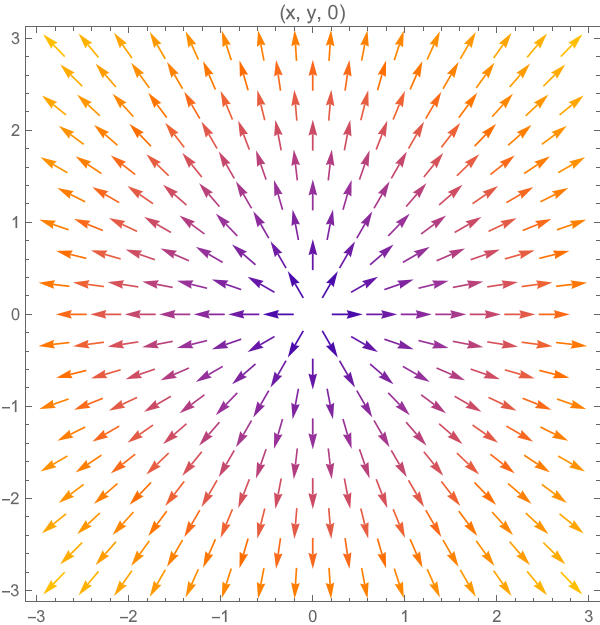
\includegraphics[width=0.45\textwidth]{../plots/VC_4_3_a.png}
    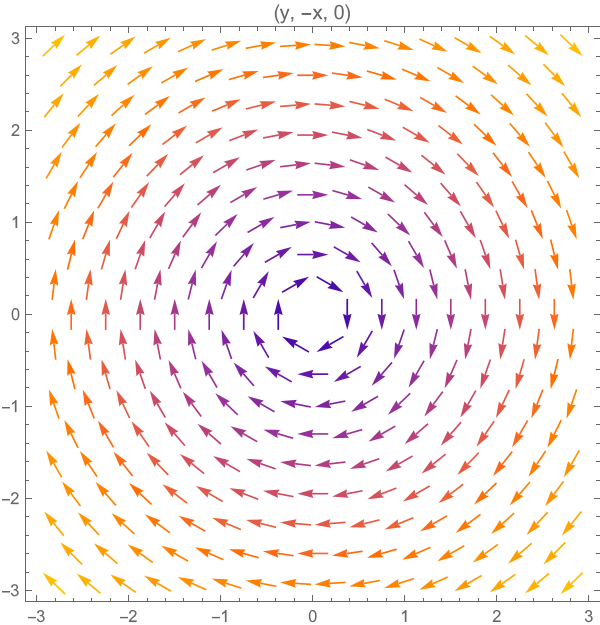
\includegraphics[width=0.45\textwidth]{../plots/VC_4_3_b.png}
\end{center}

It is easy to calculate that

\begin{equation}
    \nabla \cdot \mathbf{A} = 2, \quad \nabla \cdot \mathbf{B} = 0
\end{equation}

The curls are given by the matrix

\begin{equation}
    \nabla \times \mathbf{A} = 
    \begin{pmatrix}
        \hat{i} & \hat{j} & \hat{k} \\
        \partial_{x} & \partial_{y} & \partial_{z} \\
        x & y & 0
    \end{pmatrix}
    =
    \mathbf{0}, \quad
    \nabla \times \mathbf{B} =
    \begin{pmatrix}
        \hat{i} & \hat{j} & \hat{k} \\
        \partial_{x} & \partial_{y} & \partial_{z} \\
        y & -x & 0
    \end{pmatrix}
    =
    (0, 0, -2)^{\intercal}
\end{equation}

$A$ is a curl-free vector field (like an electric field), and $B$ is a divergence-free vector field (like a magnetic field).
\qed


\problem{4}{}
The curl of $\mathbf{A}$ is:

\begin{equation}
    \nabla \times \mathbf{A} = 
    \begin{pmatrix}
        \hat{i} & \hat{j} & \hat{k} \\
        \partial_{x} & \partial_{y} & \partial_{z} \\
        y & -x & z
    \end{pmatrix}
    =
    (0, 0, -2)^{\intercal}
\end{equation}

The area integral of the curl on the hemisphere is given by:

\begin{equation}
    \int_{S} (\nabla \times \mathbf{A}) \cdot \mathrm{d}\mathbf{a} = -2\int_{S} \mathrm{d}a_{z} = -2\pi
\end{equation}

The curve $C$ bounding the hemisphere is given by $\left\{ (r, \theta, 0) \vert r = 1, \theta \in [0, 2\pi] \right\}$. The line integral of $\mathbf{A}$ along the curve is given by:

\begin{equation}
    \int_{C} \mathbf{A} \cdot \mathrm{d}\mathbf{l} = \int_{0}^{2\pi} -r^{2} \sin^{2}{\theta} - r^{2} \cos^{2}{\theta} \, \mathrm{d}\theta = -2\pi
\end{equation}

as expected from Stokes' theorem.
\qed


\problem{5}{}
Still using polar coordinates, the line integral is given by:

\begin{equation}
    \int_{C} \mathbf{A} \cdot \mathrm{d}\mathbf{l} = \mistake{\int_{0}^{2\pi} -r \sin^{2}{\theta} - (3 + r\cos{\theta}) \cos{\theta} \, \mathrm{d}\theta} = -2\pi r = -2\sqrt{2} \pi
\end{equation}

\begin{correction}
    \begin{equation}
        \int_{C} \mathbf{A} \cdot \mathrm{d}\mathbf{l} = \int_{0}^{2\pi} -r^{2} \sin^{2}{\theta} + (3 + r\cos{\theta}) r \cos{\theta} \, \mathrm{d}\theta = -4\pi
    \end{equation}
\end{correction}

\qed


\problem{6}{}
Operating in cylindrical coordinates, a point at radius $r$ has the velocity $\mathbf{v} = \omega r \hat{\phi}$. The divergence and curl of $\mathbf{v}$ are:

\begin{equation}
    \nabla \cdot \mathbf{v} = 0, \quad \nabla \times \mathbf{v} = 2\omega \hat{z}
\end{equation}

$\mathbf{v}$ being divergence-free means that the 'flow' is purely rotational, so a particle cannot change its $r$ as expected from a rigid body. The flow cannot be represented by a potential field, as the curl is non-zero.
\qed


\problem{7}{}

\begin{equation}
    \nabla \times (\nabla \phi)
    =
    \begin{pmatrix}
        \hat{i} & \hat{j} & \hat{k} \\
        \partial_{x} & \partial_{y} & \partial_{z} \\
        \phi_{x} & \phi_{y} & \phi_{z}
    \end{pmatrix}
    =
    \mathbf{0}
\end{equation}

as the double partial derivatives cancel.

\begin{equation}
    \nabla \cdot (\nabla \times \mathbf{A})
    =
    \nabla \cdot \begin{pmatrix}
        \partial A_{z}/\partial y - \partial A_{y}/\partial z  \\
        \partial A_{x}/\partial z - \partial A_{z}/\partial x  \\
        \partial A_{y}/\partial x - \partial A_{x}/\partial y
    \end{pmatrix}
    = 0
\end{equation}
\qed


\problem{8}{}
First express $\mathrm{d}\mathbf{r}$ in terms of $\mathrm{d}t$:

\begin{equation}
    \mathrm{d}\mathbf{r} = (2t, 2, 2t^{2})^{\intercal} \mathrm{d}t
\end{equation}

The line integrals are given by:

\begin{equation}
    \int_{C} \phi \, \mathrm{d}\mathbf{r} = \int_{0}^{1} 4t^{9} (2t, 2, 2t^{2})^{\intercal} \, \mathrm{d}\mathbf{r} = (8/11, 8/10, 8/12)^{\intercal}
\end{equation}

\begin{equation}
    \int_{C} \mathbf{F} \times \mathrm{d}\mathbf{r} = \int_{0}^{1} 2 (-t^{4} - t^{5}, -t^{5}, 2t^{3} + t^{4})^{\intercal} \, \mathrm{d}\mathbf{r} = (-11/15, -1/3, 7/5)^{\intercal}
\end{equation}
\qed


\problem{9}{}

\begin{equation}
\begin{split}
    a_{i} b_{j} c_{i} &= (\mathbf{a} \cdot \mathbf{c}) \mathbf{b} \\
    a_{i} b_{j} c_{j} d_{i} &= (\mathbf{a} \cdot \mathbf{d}) (\mathbf{b} \cdot \mathbf{c}) \\
    \delta_{ij} a_{i} a_{j} &= \mathbf{a} \cdot \mathbf{a} \\
    \mistake{\delta_{ij} \delta_{ij}} &= 1 \\
    \epsilon_{ijk} a_{i} b_{k} &= \mathbf{b} \times \mathbf{a} \\
    \epsilon_{ijk} \delta_{ij} &= 0 \\
\end{split}
\end{equation}

\begin{correction}
    \begin{equation}
        \delta_{ij} \delta_{ij} = \delta_{ii} = 3
    \end{equation}
\end{correction}

\qed


\problem{10}{}
\begin{equation}
\begin{split}
    \nabla r^{n} &= \sum_{i} \frac{\partial }{\partial x_{i}} \left( \sum_{j} x_{j} \right)^{n/2} \hat{e}_{i} \\
    &= \sum_{i} \frac{n}{2} \left( \sum_{j} x_{j} \right)^{n/2 - 1} \frac{\partial \sum x_{j}^{2}}{\partial x_{i}} \hat{e}_{i} \\
    &= \sum_{i} \frac{n}{2} \left( \sum_{j} x_{j} \right)^{n/2 - 1} 2x_{i} \hat{e}_{i} \\
    &= n r^{n-2} \mathbf{r} \\
    &= n r^{n-1} \hat{r}
\end{split}
\end{equation}

\begin{equation}
    \nabla (\mathbf{a} \cdot \mathbf{r}) = \sum_{i} \frac{\partial }{\partial x_{i}} \left( \sum_{j} a_{j} x_{j} \right) \hat{e}_{i} = \sum_{i} a_{i} \hat{e}_{i} = \mathbf{a}
\end{equation}
\qed


\problem{11}{}

\subproblem{a}

\begin{equation}
    \nabla \cdot \mathbf{r} = \partial_{x_{i}} x_{i} = 3
\end{equation}

\begin{equation}
    \nabla \times \mathbf{r} = \epsilon_{ijk} \partial_{x_{j}} x_{k} \hat{e}_{i} = \mathbf{0}
\end{equation}

\subproblem{b}

\begin{equation}
\begin{split}
    \nabla \cdot (r^{n} \mathbf{r}) &= \sum_{i} \partial_{x_{i}} \left[ \left( \sum x_{j}^{2} \right)^{n/2} x_{i} \right] \\
    &= \sum_{i} \left( \sum x_{j}^{2} \right)^{n/2} + x_{i} \frac{n}{2} \left( \sum x_{j}^{2} \right)^{n/2 - 1} 2x_{i} \\
    &= \mistake{r^{n} + n r^{n-1}}
\end{split}
\end{equation}

\begin{correction}
    \begin{equation}
    \begin{split}
        \nabla \cdot (r^{n} \mathbf{r}) &= \sum_{i} \partial_{x_{i}} \left[ \left( \sum x_{j}^{2} \right)^{n/2} x_{i} \right] \\
        &= \sum_{i} \left( \sum x_{j}^{2} \right)^{n/2} + x_{i} \frac{n}{2} \left( \sum x_{j}^{2} \right)^{n/2 - 1} 2x_{i} \\
        &= 3r^{n} + n r^{n} \\
        &= (3 + n) r^{n} \\
    \end{split}
    \end{equation}
\end{correction}

\begin{equation}
    \nabla \times (r^{n} \mathbf{r}) = \epsilon_{ijk} \partial_{x_{j}} (r^{n} x_{k}) \hat{e}_{i} = \epsilon_{ijk} r^{n-1} n x_{j} x_{k} \hat{e}_{i} = n r^{n-2} (\mathbf{r} \times \mathbf{r}) = \mathbf{0}
\end{equation}

\subproblem{c}

\begin{equation}
    \nabla \cdot [(\mathbf{a} \cdot \mathbf{r}) \mathbf{b}] = \sum_{i} \partial_{x_{i}} \left( \sum_{j} a_{j} x_{j} \right) b_{i} = \sum_{i} a_{i} b_{i} = \mathbf{a} \cdot \mathbf{b}
\end{equation}

\begin{equation}
    \nabla \times [(\mathbf{a} \cdot \mathbf{r}) \mathbf{b}] = \epsilon_{ijk} \partial_{x_{j}} \left( \sum_{l} a_{l} x_{l} \right) b_{k} \hat{e}_{i} = \epsilon_{ijk} \delta_{lj} al b_{k} \hat{e}_{i} = \mathbf{a} \times \mathbf{b}
\end{equation}

\subproblem{d}

\begin{equation}
    \nabla \cdot (\mathbf{a} \times \mathbf{r}) = \partial_{x_{i}} \epsilon_{ijk} a_{j} x_{k} = 0
\end{equation}

\begin{equation}
    \nabla \times (\mathbf{a} \times \mathbf{r}) = \epsilon_{ijk} \partial_{x_{j}} (\epsilon_{klm} a_{l} x_{m}) \hat{e}_{i} = \epsilon_{kji} \epsilon_{klm} a_{l} \delta_{mj} \hat{e}_{i} = \delta_{il} \delta_{jm} a_{l} \delta_{mj} \hat{e}_{i}  - \delta_{im} \delta_{jl} a_{l} \delta_{mj} \hat{e}_{i} = \mistake{\mathbf{a}}
\end{equation}

\begin{correction}
    \begin{equation}
        \nabla \times (\mathbf{a} \times \mathbf{r}) = \delta_{il} \delta_{jm} a_{l} \delta_{mj} \hat{e}_{i}  - \delta_{im} \delta_{jl} a_{l} \delta_{mj} \hat{e}_{i} = 3 a_{i} \hat{e}_{i} - a_{i} \hat{e}_{i} = 2 \mathbf{a}
    \end{equation}
\end{correction}
\qed


\problem{12}{}
\begin{equation}
    \nabla \times (\nabla \phi) = \nabla \times (\partial_{x_{i}} \phi_{i} \mathbf{e}_{i}) = \epsilon_{ijk} \partial_{x_{j}} \partial_{x_{k}} \phi_{k} \mathbf{e}_{i}
\end{equation}

Note that $\epsilon_{ijk} \partial_{x_{j}} \partial_{x_{k}} = \epsilon_{ikj} \partial_{x_{k}} \partial_{x_{j}} = - \epsilon_{ikj} \partial_{x_{k}} \partial_{x_{j}} = 0$. Therefore, $\nabla \times (\nabla \phi) = \mathbf{0}$.

\begin{equation}
    \nabla \cdot (\nabla \times \mathbf{A}) = \nabla \cdot (\epsilon_{ijk} \partial_{x_{j}} A_{k} \mathbf{e}_{i}) = \epsilon_{ijk} \partial_{x_{i}} \partial_{x_{j}} A_{k} = 0
\end{equation}

\end{document}